\chapter{INTRODUCTION}
\section{Background Information}
The use of computer and computing devices, in the recent decade has seen greater development more than any known time in history. This cuts across all spheres of endeavour. This is seen in the use of different and diverse computer-vision and artificial intelligence based tools in all works of life. According
\citep{ghazalComputerVisionSmart2024}, Vision-based intelligent systems have made way to practically every aspect of modern human life. These systems combine computer vision, artificial intelligence (AI), and machine learning technologies and allow machines to mimic human visual and cognitive abilities to make informed decisions about the task at hand. Computer vision technology is used to process and interpret visual information from the surrounding environment while the artificial intelligence (AI) technologies along with machine learning algorithms are used for recognizing patterns and predicting actions.

According to \citep{VULLAGANTI2025147} Precision agriculture is one such practice, which uses advanced technologies and data-driven approaches to aid decision making and optimize crop production. For crop growth, nutrients are the most crucial and most used inputs. SSNM is an effective precision agriculture practice for efficient application of nutrients. This involves identifying the spatio-temporal variability of nutrient status and deficiencies in agricultural fields and applying fertilizers accordingly at variable rates. Principles and practices of SSNM are aided by the 4 R nutrient stewardship concept, namely, 
\begin{enumerate}
	\item Using the right fertilizer,
	\item Applying at the right time
	\item Using the right source, and 
	\item Adopting the right method
\end{enumerate}

Early identification of the pathogen type of plant infection is of high significance for disease control. Various methods are used to diagnose pathogens of disease on plant. This article discusses the review of the literature data on traditional methods for diagnosis of plant pathogens, such as visual observation, microscopy, mycological analysis, and biological diagnostics or the use of indicator plants. Rapid and reliable detection of plant disease and identification of its pathogen is the first and most important stage in disease control. Early identification of the cause of the disease allows timely selection of the proper protection method and ensures prevention of crop losses. There are a number of traditional methods for identifying plant diseases, however, in order to ensure the promptness and reliability of diagnostics, as well as to eliminate the shortcomings inherent in traditional diagnostics, in recent years, new means and technologies for identifying pathogens have been developed and introduced into practice. As well as the article provides information on such innovative methods of diagnosis of diseases and identification of their pathogens, which are used widely in the world today, such as immunodiagnostics, molecular-genetic (and phylogenetic) identification, mass spectrometry. \citep{Khakimov_2022}

% Traditional disease detection techniques which normally includes laboratory tests and expert consultation can be slow, costly and limited in scope. According to (Lokesh et al.). ML offers a more efficient and accurate solution, enabling early disease detection and timely intervention.

\paragraph*{} Artificial intelligence algorithms are trained on large datasets of image or other data forms related to the plant diseases. Artificial intelligence algorithms learn to understand and recognize patterns and features associated with the differing diseases, making it possible for the Artificial Intelligence models to predict the presence and severity of disease in new, unseen data.

\paragraph*{} There are many types of ML algorithms that can be employed for Ugu disease detection. These include image processing technique, deep learning modelss (like Convolutional Neural Networks - CNNs), and other classifiers. In this, work it is intended to you deep learning and or image processing techniques. 

\paragraph*{} Faster detection: ML algorithms can process images and data rapidly, enabling early disease detection and timely interventions, according to ResearchGate Improved accuracy: ML models can often outperform traditional methods in terms of accuracy, reducing the risk of misdiagnosis and enabling more precise interventions, according to ResearchGate. Increased production: By enabling early and accurate disease detection, ML can help farmers take timely action to prevent crop loses and increase productivity. 

\paragraph*{} Data availability: Training ML models requires large and diverse datasets of plant disease images or data, which may be challenging to obtain. Data quality: The quality of the data used to train ML models can significantly impact their performance, and poor quality data can lead to inaccurate predictions. Generalisation: ML models may struggle to generalise to new or unseen conditions, such as different plant species or environmental factors, according to {\bfseries Diva Portal}

\paragraph*{} 
Early disease detection: ML can be used to identity disease symptoms at their earliest stages, allowing for timely interventions and preventing the spread of diseases. Disease classification: ML models can be trained to classify different types of plant diseases, aiding in accurate diagnosis and targeted treatment. Disease severity assessment: ML can be used to assess the severity of plant diseases, helping farmers determine the approximate treatment strategies. Predicting disease outbreaks: By analysing historical data and environmental factors. ML can be used to predict the likelihood of disease outbreaks, allowing for proactive measures to be taken, according to ResearchGate.

\paragraph*{} Image-based detection: ML algorithm can analyse images of plant leaves to identify disease symptoms, such as lesions, discolouration and other visual clues.

\paragraph*{}Pumpkin is the name given to a group of plant species in the genus Cucurbita, including Cucurbita pepo, Cucurbita mixta, Cucurbita maxima, and Cucurbita moschata. It is grown primarily as a vegetable or ornamental plant.
%
Pumpkins have long-running, bristled stems, large deeply-lobed leaves often containing white blotches, and yellow or orange flowers separated into male and female types on the same plant. The fruit (for the group) is variable in shape and color but is often white [see][]~\ref{fig:ike_ugu}, cream, or green, containing about 70\% flesh and several large white seeds.
\newline

Ugu (fluted pumpkin) is a member of pumpkin family. And according to \citep{PumpkinDiseasesPests}, Pumpkin plants are short-lived annual or perennial vines with branching tendrils and broad lobed leaves. 

%The plant produces large yellow or orange flowers and a pepo fruit (berry with a thick rind) known as a pumpkin. The fruit can range greatly in size, from miniature pumpkins weighing a few ounces to giant pumpkins which can reach over 75 lbs (34 kg). The skin of the pumpkin is usually ribbed and is usually orange in color although some varieties are green, grey, yellow, or red. Pumpkin plants are usually grown as annuals, surviving one growing season and the vines are capable of reaching 15 m (50 ft) in length if vines are allowed to root. Pumpkin may also be referred to as squash or marrow and is believed to have originated in Mexico and South America.

% Start 
\citep{ifyInterestingFactsYou2024} said these about Ugu, fluted pumpkin.
Fluted pumpkin, also known as “ugu” leaves, originates from West Africa, particularly Nigeria. Its scientific name is Telfairia occidentalis. This leafy vegetable is a staple in Nigerian cuisine and is widely cultivated for its culinary and nutritional benefits.

The nature of fluted pumpkin is characterized by its distinctive fluted stem, large dark green leaves, and tendrils. It is a climbing plant that thrives in tropical climates, and its cultivation involves providing adequate sunlight and well-drained soil.

The importance of fluted pumpkin, or ugu leaves, lies in its nutritional richness. It is a good source of essential vitamins such as A and C, calcium, iron, and other micronutrients. The leaves are commonly used in soups, stews, and various local dishes, contributing both flavor and nutritional value to the diet.

Beyond its culinary uses, fluted pumpkin holds cultural significance and is often used in traditional medicine for its perceived health benefits. Additionally, the cultivation and trade of ugu leaves contribute to the economic well-being of farmers in the region.

Some Facts and Nutritional Benefits of Fluted Pumpkin Leaves or Vegetables include;
\begin{description}
	\item[Good Source of Dietary Fibre:] Fluted pumpkin leaves are a source of dietary fiber that helps maintain the digestive system’s health. It plays an essential role in improving digestion, thereby reducing health conditions like irritable bowel movement, constipation, and those caused by indigestion problems like ulcers and gastroparesis.
	
	\item[Maintains the Body Tissues:] The vitamin contents in this vegetable help maintain healthy tissues, cells, membranes, and skin and treat wounds in the case of vitamin C. The protein in fluted pumpkin leaves alsoleaves also helps improve and maintain the body tissues, which include the connective tissues, muscles, and nervous systems.
	
	\item[Rich in Antioxidants:] They are rich in alkaloids, resins, hydrocyanic acid, tannins, and flavonoids, powerful antioxidants that offer some immune system and anti-inflammatory benefits. Foods rich in antioxidants are known to be effective in preventing cancer and other associated health conditions like ulcers due to their ability to avoid the damages that oxidative stress should have caused in the body.
	
	\item[Balances the Hormones:] 
	Vegetable is known to have high protein content. Ugu contains the protein needed for hormone balancing; tissue repairs and regulates the acidities of body cells and organs. Consuming fluted pumpkin leaves is essential, as their protein content will also help improve the body cells and replace broken ones.
	
	\item[Serve as an Anti-Diabetic Agent:] It has an anti-diabetic effect, which means it can treat diabetes mellitus by reducing glucose in the blood. It is possible due to the content of polysaccharides and ethyl acetate, which have effectively lowered blood sugar levels. They also effectively promote glucose tolerance and serum insulin. The extract of Ugu leaves has proved effective in this case, and it has been used as an anti-diabetic agent to regulate the blood glucose level.
	
	\item[Improves Blood Production:] Fluted pumpkin leaves are always recommended for patients who suffer from a shortage of blood due to certain illnesses; the presence of iron and other essential minerals contributes to boosting blood in the body system and prevents anemia. For the effectiveness of helping boost blood production, it is recommended to be pounded, then strain the mashed vegetable to collect the liquid/juice.
	
	\item[Improves the Bones and Teeth:] Fluted pumpkin vegetables contain a good amount of calcium needed to maintain healthy bones and teeth and keep the skeletal systems functioning normally. It also contains magnesium, which is vital in making the bone firm and strong. It might be surprising to say that calcium is almost ineffective to bones without magnesium as it helps the adequate absorption of calcium by the bones. Ugu also has potassium as one of the minerals it contains, which also helps maintain bone mineral density, which helps to make the calcium content in the bones intact, avoiding the leaching of the mineral. It helps to prevent osteoporosis, which affects the bones, especially in the aged.
	
	\item[Treat Convulsion:] Ugu leaves have been found effective in treating convulsions in children. It becomes medicinal when sliced and mixed with coconut water and a small amount of salt. Scientifically, there might be no proof of this, but it was used hundreds of years ago to treat high fever and convulsion and remedy many other health conditions.
	
	\item[Effective for Weight Loss:] Foods that help in weight loss are recommended for their effectiveness in weight management. Vegetables such as fluted pumpkin leaves contain a high amount of dietary fiber, which can help you lose weight as it makes you fuller and lowers your appetite. It contains little or no calories, eliminating the chances of storing more calories in the body.
	
	\item[Promotes Fertility:] Fluted Pumpkin leaves have been used locally to treat infertility issues in both men and women. Its content of many vital nutrients and compounds has proven effective in its use to boost/improve sperm count in men and the overall functioning of their testicles. It boosts fertility in women and improves post-pregnancy health as it helps the nursing mother adequately feed their babies by increasing breast milk production.
	
	\item[Can Improve Memory:] Fluted pumpkin leaves, just like most green leafy vegetables, contain certain compounds that help to improve memory. It also contains vital nutrients such as vitamins and magnesium, which aid in improving and normal functioning of the brain and nervous system. It can help to Improve cognitive reasoning, memory loss (Dementia), and other health conditions associated with memory health, such as Alzheimer’s disease.	
\end{description}
% Finish

% \paragraph*{} Ugu leave (botanical name, Telfaira occidentalis) is also known as fluted pumpkin and is a green-leafy vegetable that originated from Nigeria. It is well planted and consumed all over the country especially in the Eastern parts of Nigeria. It is also well consumed in the Western and Northern parts of Nigeria. Ugu is loaded with a lot of vitamins like Vitamin A, B2, C, and E, minerals like Calcium, Iron, Potassium, Magnessium, Folic acid, Manganese, dietary fibre and other micro nutrients. It is also loaded with other health benefits like hormone balancing, male-female reproductive boosting properties. Dark leafy greens like Ugwu (ugu) are rich in Vitamins A, C and E, as well as essential minerals like iron and magnesium. These nutrients are crucial for maintaining healthy skin and preventing premature ageing (classiscauthor, 2024).

%\paragraph*{} Have you ever heard about the positive impact of Ugu vegetable's leaves on your health? This vegetable has tons of Vitamins  and minerals, which help your body to stay healthy and skin to remain smooth, (Adriama, 2017). Hence there exists the potential to harness the rich content of Ugu as a natural source of nutrients and other essential compounds for the production of organic and organic-based beauty products. Also, it could serve as a constituent for the production of supplements by the pharmaceutical firms. (Eseyin et al.)

%\paragraph*{} According to (Kayode and Kayode, 2010) several medicinal uses of the fluted pumpkin (Telfairia occidentalis) in traditional medicine have been documented. Although, many of these claims are yet to be validated by scientific researchers, a review of some investigated therapeutic activities of the plant are highlighted in this article. Experimental works done on Telfaira occidentalis especially in the field  of Biochemistry were retrieved via Google search on the internet and studied carefully to identify any therapeutic activity reported on Telfaira occidentalis. It can be inferred that the ability of the plant to combat certain diseases may be due to its antioxidant and antimicrobial properties and its minerals (especially Iron), vitamins (especially vitamin A and C) and high protein contents. We therefore conclude that with further chemical manipulation and clinical investigations numerous drugs designs could emerge from the plant.

%\paragraph *{} According to (Opara and Okoronkwo, 2021) it is also a source of oil used for cooking and making soaps, margarine, paint and varnishes. According to this, vegetable oil is being extracted from this wonderful leaf for cooking and soap making, margarine (a consumable) and paints, but who could have believed this? Varnishes are also produced from Ugu leaf.

%\paragraph*{} The production process of Ugu involves the making of the planting platform (ridge, bed or mounds) planting with the seed and facing the cortex of the seed down. The planting, preferably by the onset of the rainy season (can also be planted all year round with access to water supply) is followed by the first cut  "i tu be onu" after about a month of sprouting and or when it must have got about more than four buds. This is to encourage more shooting out from these buds. Then regular or constant weeding as at when needed (weed monitoring and management). Then also regular checks for diseases / inspection and or nutritional issues. (NATURE'S HERITAGE NETWWORKS, 2021)
Ugu leaf has a lot of benefit to the healthy leaving of man. I personally have heard of recovered eye-sight case by constant consumption of Ugu leaf and nturukpa (another leaf common to the eastern Nigeria). 
According to , \citep{olagunjuFlutedPumpkinLeaf2016} \begin{quotation}
	Igbos in South East Nigeria call it Ugu and can barely live without it. But why should they when it has numerous health benefits?
	Telfairia occidentalis, as it is scientifically called is a tropical vine grown in West Africa as a leaf vegetable and for its edible seeds. Common names for the plant include fluted gourd, fluted pumpkin, and ugu and it is mainly cultivated in Nigeria. Ugu is used primarily in soups and herbal medicines though its fruits are edible, its seeds produced by the gourd, are high in protein and fat, and can, therefore contribute to a well-balanced diet.
	However, recently, nutritionists have been hammering on the wonders of juicing and how it benefits the body. Thus, more health conscious people are tilting towards juicing now more than before with the claim that anything can be juiced and juices are easier absorbed into the body system than solid foods. So, "while most of us have been using our ugu leaves in varieties of soups, some people have been juicing it for direct maximum nourishments,” nutritionist Efemena Okeze says.
	
	As the name suggests, pumpkin juice is an extract from fresh pumpkin leaves and has several health benefits. And as such, it can be used as a healthy substitute for carbonated drinks.
	
	According to Grace Tinkola, an undergraduate at a South-West University, “I grew up drinking ugu juice sweetened with malt drink because of my mother. Then, I thought mother was just singing its praises to get us to drink it. But now that I am grown, I keep thanking my mom for forcing my siblings and me to make it a habit. It is a very healthy way of life but now I take it without the malt drink.”
	
	Fluted pumpkin leaves are rich in potassium, calcium, iron and some Folic acid. They also contain a healthy amount of Vitamin A, Vitamin C, Vitamin E, Thiamin, Niacin, vitamin B6, Folate, Iron, magnesium and phosphorus, and are a very good source of dietary fibre, riboflavin, Copper and Manganese.
	
	The anti-oxidants such as alpha-carotene and Beta–carotene contained in the leaves help to slow down ageing process and also help to eliminate free radicals which are responsible for growth of cancer. The iron contained in the leaves helps to improve blood levels as well as prevent anaemia. This means that the leaves are good for people with heavy menstrual periods, pregnant women or people with poor absorption due to gut diseases such as, coeliac disease and Crohn’s disease. Those who eat poor or restricted diets, those with red blood cell problems such as thalassaemia, sickle cell anaemia and those with bone marrow problems and leukaemia will benefit from it as well.
	
	Vitamin C in the leaves helps to heal wounds, form scar tissue, and maintain healthy bones, skin, and teeth. It is rich in vitamin E, which promotes a healthier skin and in turn slows down the aging of the skin.
	
	Carotene, which converts to vitamin A in the body is present in the leaves and aside from the vision benefits in Vitamin A that the leaves provide, there are also numerous skin benefits.
	
	
	Taiwo Olayinka, a beautician and owner of pretty concepts studio, explains the importance of the vitamins C, E and beta-carotene on the skin thus: “Vitamin C, also known as ascorbic acid, is important for the production of collagen, a protein that aids in the growth of cells and blood vessels and gives the skin its firmness and strength; helps to create scar tissue and ligaments; and aids in skin repair.
	
	“Vitamin C is an antioxidant and slows the rate of free-radical damage to collagen that can contribute to dry skin, fine lines and wrinkles. Vitamin E is an antioxidant that protects and repairs your skin and can help prevent premature ageing of your skin and damage to your DNA.”
	
	The Journal of Investigative Dermatology reported in February 2005 that people who take vitamins C and E in the long term reduced their sunburns from exposure to UVB radiation. Further, researchers saw a reduction of factors linked to DNA damage within skin cells.
	
	Beta-carotene according to nutritionists is a strongly coloured pigment that imparts the yellow and orange fruits and vegetables their rich hues. Once ingested, it gets converted into vitamin A (retinol) which performs several biological functions within the body. Vitamin A also acts as an antioxidant that protects cells from the damaging effects of harmful free radicals.
\end{quotation}

Ugu leaf (Talifairia occidentalis) is such an amazing gift to humanity that many people have different testimonies about it. Credit to \citep{7AmazingUses}, the following are the leaf, gourd and seed of Ugu leaf (fluted pumpkin): 

\begin{figure}[!h]
	\centering	
	\label{fig:ugu_leaf}
	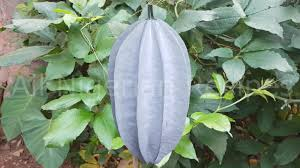
\includegraphics{ugu_gourd.jpeg}
	\caption{Ike Ugu or Ugu gourd} 

\end{figure}
\newpage
\begin{figure}[!h]
	\centering
	\label{fig:ugu_leaf}
	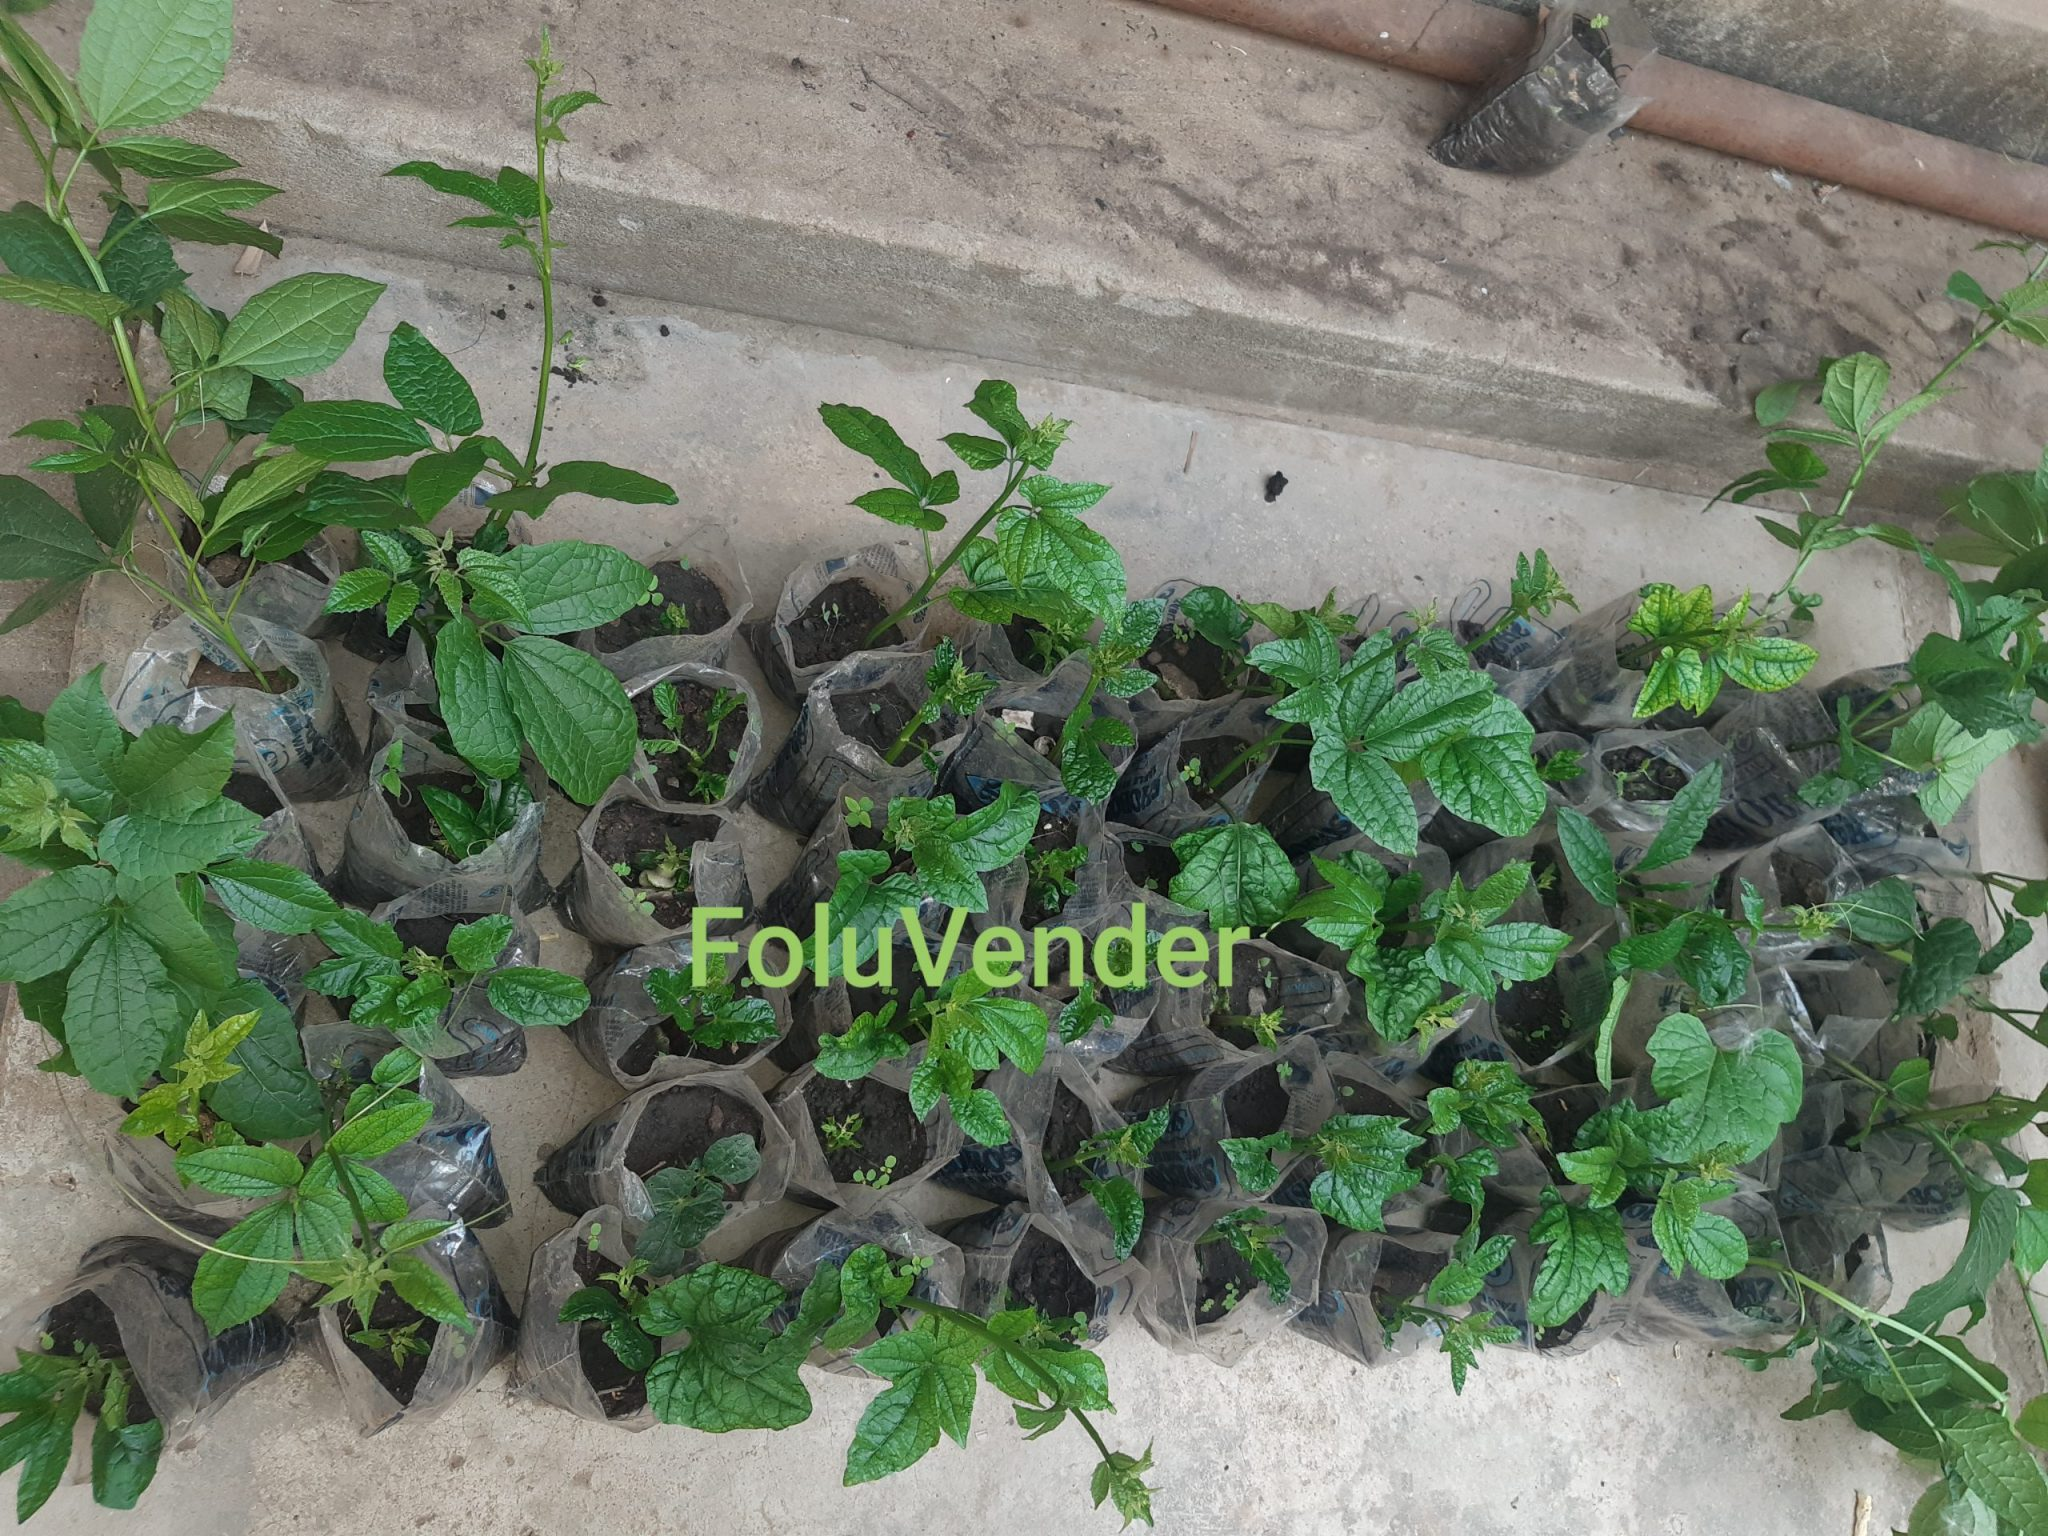
\includegraphics[scale=.20]{ugu_leaf.jpg}
	\caption{Ugu leaf. Credit: farmsquare.ng} 
	
\end{figure}

\begin{figure}[!h]
	\centering
	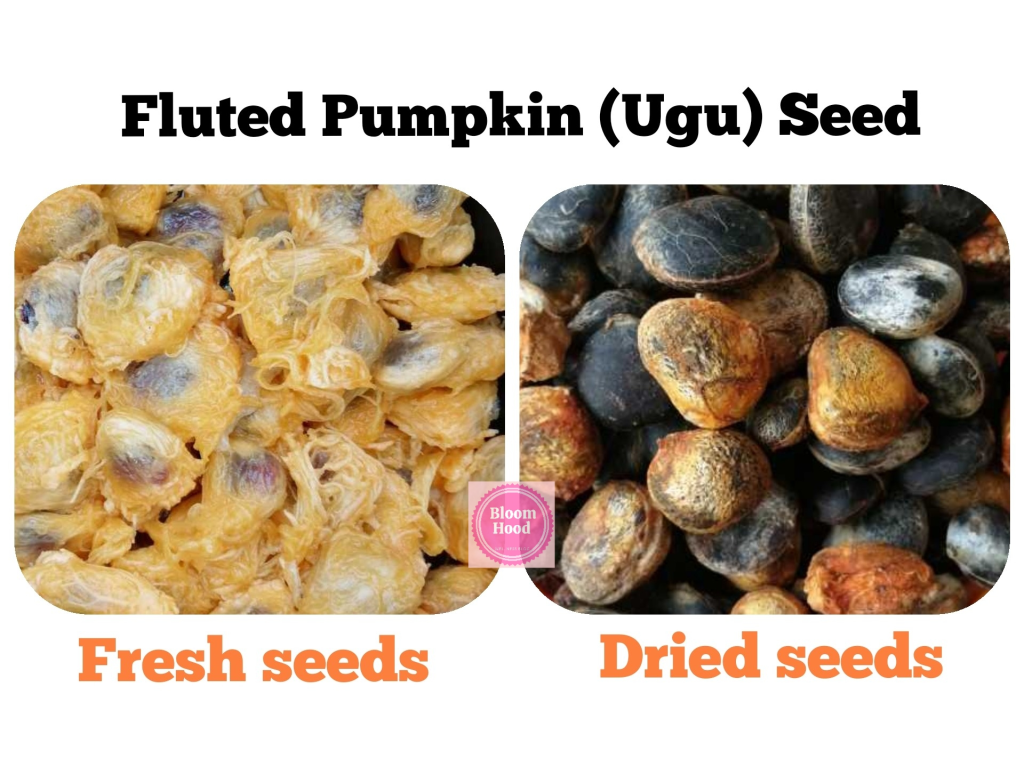
\includegraphics[scale=.40]{ugu_seed.png}
	\caption{Ugu seed. Credit: farmsquare.ng} 
	\label{fig:ugu_seed}
\end{figure}

\newpage
\section{Problem Statement}
Develop an ML/AI based system for the early and accurate detection of various Ugu leaf diseases as listed in section \ref{ref:ugu_diseases}, leveraging diverse image datasets, and advanced algorithms to improve farm production efficiency and better crop yield.

\section{Objectives}
The objectives of the study is primarily to develop an accurate, efficient and robust system for identifying the diseases mentioned in \ref{ref:ugu_diseases} particularly in its early stage. This early detection is very important for prompt management intervention and control and can assist in reduction of crop losses and prevent the spread of the disease(s).

\section{Research Questions}
\begin{itemize}
	\item What is the accuracy of using image processing to identify and classify different Ugu leaf diseases?
	\item How does image processing and classification compare to traditional methods of Ugu leaf disease detection?
\end{itemize}


\section{Justification of the Study}
\begin{itemize}
	\item Existing methods for vegetables, fruits and other plant's leaf diseases identification suffer from low accuracy, posing a huge challenge for precise classification.
	
	\item To proffer suitable solutions to identified Ugu (leaf) disease.
	
	\item The importance of the study is to find an easier and prompt method of disease detection in the farm. This will reduce loss due to disease in the farm as the cosmetic and pharmaceutical industries have standard qualities they look out for and purchase.
\end{itemize}

\section{Scope of The Study}
The scope of the study is to find out how ML/AI (machine learning / artificial intelligence) can be used for only disease detection and classification and treatment suggestion / recommendation in a large scale Ugu farm of the following diseases of fluted pumpkin {\bfseries 
	\begin{itemize}
		\item Downy mildew
		\item Powdery disease
		\item Mosaic disease
		\item Bacterial leaf spot
	\end{itemize}
} \label{ref:ugu_diseases}